\documentclass[a4paper]{article}

%% Language and font encodings
\usepackage[english]{babel}
\usepackage[utf8]{inputenc}
\usepackage{tabu}
\usepackage[T1]{fontenc}
\usepackage{enumitem}


%% Sets page size and margins
\usepackage[a4paper,top=3cm,bottom=2cm,left=3cm,right=3cm,marginparwidth=1.75cm]{geometry}

%% Useful packages
\usepackage{amsmath}
\usepackage{graphicx}
\usepackage{fancyhdr}

%% Title
\title{\textbf{Playing card detection}\\ PlayCDC\\Object recognition and image understanding lecture}
\author{Frank Gabel and Daniel Gonzalez}

\date{15.07.2018}

\begin{document}
\maketitle
\section{Abstract}
With the capabilities of upcoming small video capturing devices in, for example, smart contact lenses with built-in cameras, whole new ways of cheating in cardgames emerge. In order to help facilitate these cheating endeavours, we implement an algorithm that detects the suits and ranks of playing cards in the field of view of a camera using the latest iteration of the YOLO object recognition algorithm.
\begin{figure}[h]
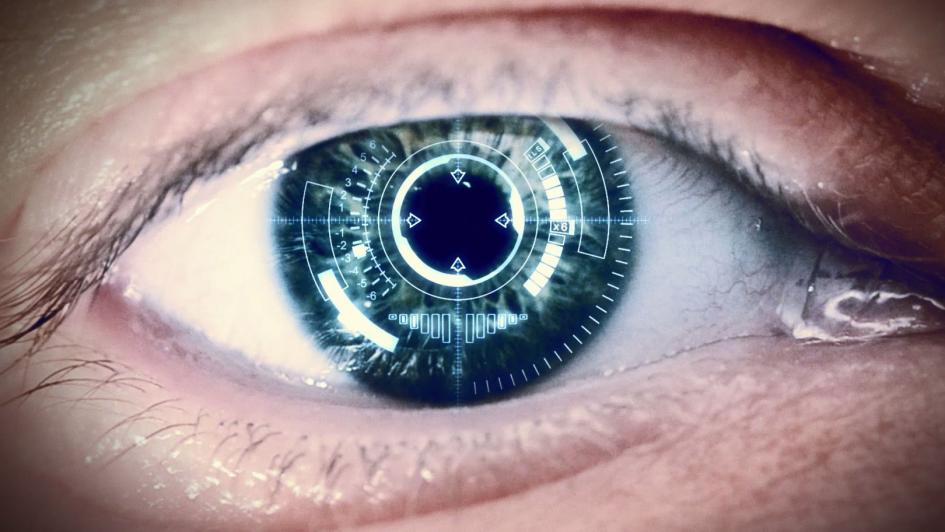
\includegraphics[scale=0.25]{contact_lense}
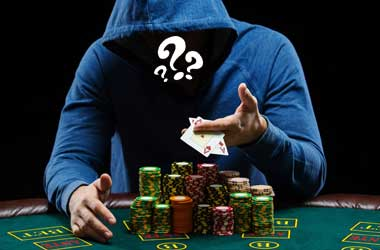
\includegraphics[scale=0.532]{poker_player}
\caption{Stock photos of an envisioned camera-equipped contact lense (left) and a mysterious black-jack player (right)}
\end{figure}
\section{Introduction}
A big topic in computer vision is the search of methods that are, given a query image, capable of answering questions like: What is present in an image? Is there a particular object in it? Where exactly in the image is this object located? Is it possible to semantically segment objects of interest in the image?
Object detection deals with detecting instances of semantic objects of a certain class (such as humans, buildings, or cars) in digital images and videos. Typically, object detection deals with two sub-taks: \textbf{object localization} using bounding boxes and \textbf{multiclass object classification} within said bounding boxes.
Sometimes, a third sub-task of \textbf{semantic object segmentation} is performed, i.e. the process of labelling objects on pixel level.\\
In this project, we use the YOLOv3 object detection algorithm (CITE) for object detection (without additional segmentation) in order to tell apart playing cards of a standard 52-part deck.

\section{Dataset}
DANIEL THAT'S YOUR PLAYGROUND, PLEASE PUT A COUPLE OF PHOTOS :)))
As there was no suitable dataset of cards to use, we decided to create it by our own.  We did this in basically three main steps to obtain at the end \textbf{(Nr. images)}images,  as well as the necessary  Bounding Box information required for training our YOLO NN.   First we had to create the data doing photos and arrange it in such a way that  we can easily use it around our workflow.  The next, we had to detect the convex hulls of the card numbers and suits and the last perform rotations/re scaling/... on the images to generate new data.\\ \\
\subsection{dataset synthesis pipeline}


\large \textbf{Data preparation} \\
\normalsize
We decided to work with a deck of 52 cards, where each card contain two times the card logo.  We took for each card 2 different photos \textbf{(TODO: check this there were not really 52)} and after this we extract the cards of the photos and re-scaled them to 600x900 pixels.  We choose this resolution arbitrary, as we though that it was a nice size to work with.
For this part, we used the selection/rotation/cropping/re-scale -tools provided by GIMP\footnote{GIMP 2.8.22 - GNU Image Manipulation Program}.
Concluding this, we proceed by detecting the convex hulls of the cards numbers and suits.  We detect the convex hulls using SciPy libraries\footnote{SciPy: Open Source Scientific Tools for Python}in a semi-automatic way, verifying for each card manually that we got the desired result \textbf{[SEE FIGURE]}.
At the last step, we saved the convex hulls as an NumPy array \textbf{(cite??)} \\ \\
\large \textbf{Data generation} \\
\normalsize
The goal in this step was to generate a big amount of new data for each card destined for training or NN. We wanted to perform image transformations, like translations, rotations and re scaling, as well as blurring and sharping to generate new data.  We decided to use the imgaug python library, because it provided a nice way to keep track of the convex hulls after doing transformations. 
\section{Related work - The object detection landscape}
FRANK TEH TANK WILL WRITE THIS
\section{Methods}
\subsection*{The YOLO approach to object detection}
The YOLO model’s novel motivation is that it re-frames
object detection as a single regression problem, directly
from image pixels to bounding box coordinates and class
probabilities. This means that the YOLO model only ”looks
once” at an image for object detection.
It works by dividing an image into $S\times S$ grid. Each grid
cell predicts $B$ bounding boxes and a confidence score for
each box. The confidence scores show how confident the
model is that there is an object in that bounding box. This
is formally defined as:



\subsubsection*{tiny YOLO-v3}

The particular architecture we used for training on our dataset is \textbf{tiny YOLOv3} which essentially is a smaller version of YOLO for constrained environments.
\begin{figure}


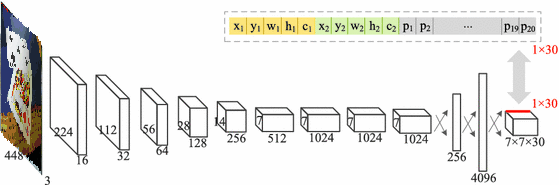
\includegraphics[width=1\linewidth]{tinyyolo}
\caption{tiny YOLO-v3 feature extractor}
\end{figure}

\subsection{Webcam deployment}
DANIEL
\subsection{Evaluation}
DANIEL - WRITE SOMETHING ABOUT MAP, YOU CAN PUT FORMULAS IN HERE LIKE A BOSS, BUILD UPON WHAT I WROTEIN THE POSTER MAYBE
\section{Results}
FRANK 
\section{Discussion}
FRANK and DANIEL
\section{Conclusion}
FRANK and DANIEL
\end{document}